\documentclass{../khlslides}


\usetikzlibrary{mindmap}

\title[Fundamenten]{Random}
\author{Fr\'ed\'eric Vogels}


\newcommand{\link}[2]{\href{#1}{\beamergotobutton{#2}}}


\begin{document}

\begin{frame}
  \titlepage
\end{frame}

\begin{frame}
  \frametitle{Random Getallen: Gebruik}
  \begin{center}
    \begin{tikzpicture}[scale=.6,
                        transform shape,
                        mindmap,
                        remember picture,
                        concept color=blue!50]
      \node[concept] {{\tt\Huge random}}
        child[grow=90] {
          node[concept] {Cryptografie}
            child[grow=30] { node[concept] {\link{http://en.wikipedia.org/wiki/Key_generation}{KeyGen}}}
            child[grow=150] { node[concept] {\link{http://en.wikipedia.org/wiki/Salt_(cryptography)}{Salt}}}
        }
        child[grow=210] {
          node[concept] {Spellen}
            child[grow=120] { node[concept] {Dobbel\-stenen} }
            child[grow=180] { node[concept] {AI} }
            child[grow=240] { node[concept] {Random levels} }
        }
        child[grow=-30] {
          node[concept] {Algoritmen}
             child[grow=60] { node[concept] {\link{http://en.wikipedia.org/wiki/Quicksort}{Quicksort}} }
             child[grow=-0] { node[concept] {\link{http://en.wikipedia.org/wiki/Ethernet}{Ethernet}} }
             child[grow=-60] { node[concept] {\link{http://en.wikipedia.org/wiki/Monte_Carlo_algorithm}{M. Carlo}} }
        };
    \end{tikzpicture}
  \end{center}
\end{frame}

\begin{frame}
  \frametitle{Probleem}
  \begin{center} \Huge
    Nondeterminisme \\[4mm]
    $\updownarrow$ \\[4mm]
    Deterministische computer
  \end{center}
\end{frame}

\begin{frame}
  \frametitle{Randomness}
  \structure{Probleem}
  \begin{itemize}
    \item Computer heeft geen ``dobbelsteeninstructie''
    \item Kan zonder externe hulp geen willekeurige getallen genereren
  \end{itemize}
  \vskip4mm
  \structure{Oplossingen}
  \begin{itemize}
    \item Gebruik maken van user input (randomheid in muisbewegingen)
    \item \link{link://en.wikipedia.org/wiki/Hardware_random_number_generator}{Hardware} gebruik makende van ruis/fotoelektrisch effect/quantumfenomenen 
    \item \textbf{Pseudorandom getallen}
  \end{itemize}
\end{frame}

\begin{frame}
  \frametitle{Pseudorandom Getallen}
  \begin{itemize}
    \item \emph{Lijken} random
    \item Resultaat van complexe berekening
  \end{itemize}
  \structure{Voorbeeld}
  \code[font size=\small,width=.9\linewidth]{rng.js}
  produceert
  \[ 1, 70, 72, 44, 50, 75, 62, 19, 55, 41, 0, 66, 77, 17, \dots \]
\end{frame}

\begin{frame}
  \frametitle{Pseudorandom Getallen}
  \structure{Probleem}
  \[ 1, 70, 72, 44, 50, 75, 62, 19, 55, 41, 0, 66, 77, 17, 58, \alert{39, 39, 39, \dots} \]
  \begin{itemize}
    \item Pseudorandom moet nog random lijken
    \item Geen herhaling
    \item Goede verdeling
  \end{itemize}
  \vskip4mm
  \structure{Oplossing}
  \begin{itemize}
    \item Gebruik maken van bestaande oplossingen
    \item Bv. \href{http://en.wikipedia.org/wiki/Mersenne_twister}{\beamergotobutton{Mersenne Twister}}
    \item JavaScript: {\tt Math.random}
  \end{itemize}
\end{frame}

\begin{frame}
  \frametitle{{\tt Math.random}}
  \begin{center}
    \begin{tikzpicture}
      \draw[thin,-latex] (-3,0) -- (6,0);
      \draw[ultra thick] (0,0) -- (2,0);
      \draw[fill=black] (0,0) circle (.05);
      \draw[fill=white] (2,0) circle (.05);
      \node[anchor=west,rotate=90] at (0,0) {\small 0};
      \node[anchor=west,rotate=90] at (2,0) {\small 0.9999\dots};
      \draw[thin] (4,-.1) -- (4,.1);
      \node[anchor=west,rotate=90] at (4,0) {\small 2};
      \draw[thin] (-2,-.1) -- (-2,.1);
      \node[anchor=west,rotate=90] at (-2,0) {\small -1};
    \end{tikzpicture}
    \vskip4mm
    {\tt Math.random()}
    \vskip4mm
    geeft getal tussen 0 (inclusief) en 1 (exclusief) terug
  \end{center}
\end{frame}

\begin{frame}
  \frametitle{Random Numbers: Dobbelsteen}
  \begin{center}
    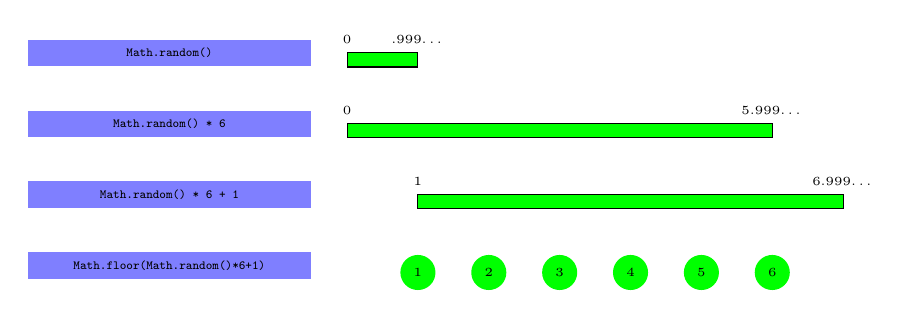
\begin{tikzpicture}[scale=.9,transform shape,rect/.style={fill=green},
                        code/.style={rectangle,minimum width=4cm,fill=blue,opacity=0.5,text opacity=1}]
      \draw[rect] (0,0) rectangle (1,0.2);
      \node[anchor=south] at (0,0.2) {\tiny 0};
      \node[anchor=south] at (1,0.2) {\tiny .999\dots};
      \node[anchor=east,code] at (-.5,0.2) {{\tt\tiny Math.random()}};

      \visible<2->{
        \draw[rect] (0,-1) rectangle (6,-0.8);
        \node[anchor=south] at (0,-0.8) {\tiny 0};
        \node[anchor=south] at (6,-0.8) {\tiny 5.999\dots};
        \node[anchor=east,code] at (-.5,-0.8) {{\tt\tiny Math.random() * 6}};
      }

      \visible<3->{
        \draw[rect] (1,-2) rectangle (7,-1.8);
        \node[anchor=south] at (1,-1.8) {\tiny 1};
        \node[anchor=south] at (7,-1.8) {\tiny 6.999\dots};
        \node[anchor=east,code] at (-.5,-1.8) {{\tt\tiny Math.random() * 6 + 1}};
      }

      \visible<4->{
        \foreach \i in {1,...,6} {
          \node[circle,fill=green] at (\i, -2.9) {\tiny\i};
        }
        \node[anchor=east,code] at (-.5,-2.8) {{\tt\tiny Math.floor(Math.random()*6+1)}};
      }
    \end{tikzpicture}
  \end{center}
\end{frame}


\end{document}



%%% Local Variables: 
%%% mode: latex
%%% TeX-master: t
%%% End: 
